\section{Prior Work and Analytic Models}\label{sec:dspmv-relatedwork}

\begin{figure*}\begin{centering}
		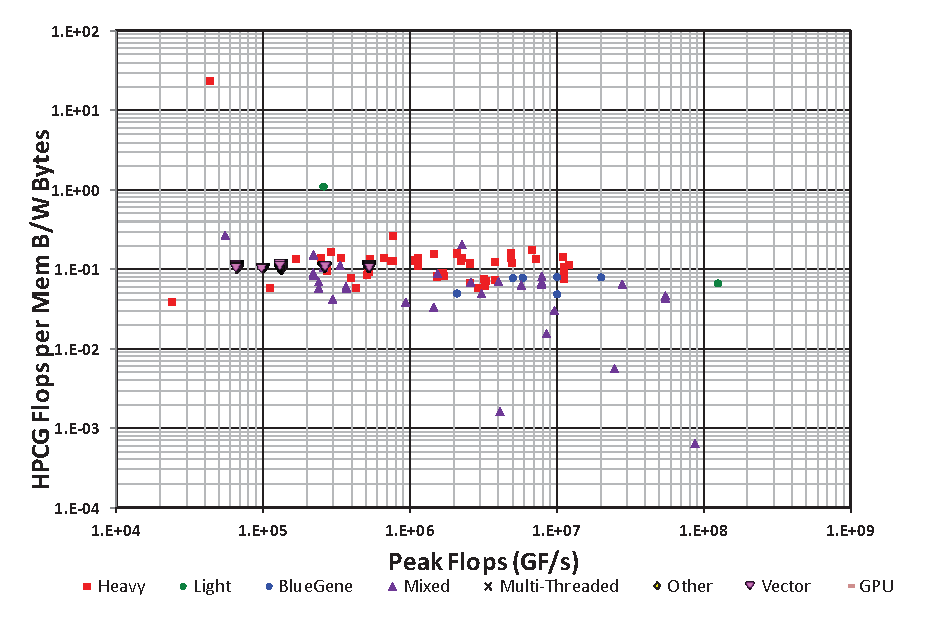
\includegraphics[scale=0.85]{figures/spmv-historical-hpcg-bw.eps}
		\caption{HPCG Flops per Byte of Memory Bandwidth vs. Peak flops.}
		\label{fig:spmv-historical-hpcg-bw}
\end{centering}\end{figure*}

The HPCG benchmark \cite{techbib:hpcg-snl-dongarra} is one that is dominated time-wise by SpMV and similar kernels. Fig. \ref{fig:spmv-historical-hpcg-bw} diagrams data taken from recent HPCG reports\footnote{http://www.hpcg-benchmark.org/}. The x-axis is the peak flops of the reported system; the y-axis is the ratio of the sustained HPCG flops to the peak bandwidth of the systems's memory (derived by determining the processing chips used and looking up their characteristics). The color and shape refer to different types of chips and systems, with the red squares representing system built from server-class chips, and the purple representing system using GPUs. 

As can be seen, this ratio is independent of the peak system flops capability. In fact it is relatively flat at about 0.1 flops per byte of memory bandwidth for heavyweight server class processor chips, and somewhat less than 0.1 for GPUs and other architectures. Since SpMV is the bulk of HPCG, this is an indication that SpMV is relatively independent of core floating point capability, and instead highly dependent on chip memory bandwidth.

A recent complexity analysis of the HPCG benchmark \cite{techbib:marjanovic2014performance} dove into HPCG performance as a function of system parameter on a kernel-by-kernel basis. The particular implementation of HPCG that was studied assumed that a sub-matrix of the total matrix was processed in each MPI rank as executed by a single core. The study rolled these numbers up into total execution time for the whole benchmark as a function of just memory bandwidth and a few network parameters. The model was extremely accurate when compared to measured HPCG data on several benchmarks.

The analysis of just the SpMV kernel within HPCG focused on just the in-core time, and computed that each sub-row as executed by a single thread on a single core required a net of the following bytes fetched from memory\footnote{The paper computed a value of 27 for the average number of non-zeros per row partition, and each non-zero required two 8-byte fetches of floating point data and one 4-byte index reference, with another 20 bytes for starting the computation of a new row.}, where $nnz_{row}$ is the average number of non-zeros per row in the row as processed by each core:

\begin{equation}\label{eqtn:BytesPerRow}
20~+~20*nnz_{row}
\end{equation}

Since each non-zero represents two flops (an add and a multiply), dividing this into $2*nnz_{row}$ yields an estimate of the bytes of bandwidth needed from memory for each flop:

\begin{equation}\label{eqtn:BytesPerFlop}
2*nnz_{row}/(20~+~20*nnz_{row}) ~=~1/(10~+~10/nnz_{row})
\end{equation}

For a $nnz_{row}$ of 27 this is about 0.096 flops per byte of bandwidth. This correlates well with HPCG, as the non-SpMV parts of HPCG require slightly more bytes per flop. Approximately 10 bytes must be accessed from memory for each flops executed.

Multiplying this by the actual sustainable memory bandwidth of a node should then estimate the sustainable flops per second for SpMV running in all the cores in that node. \cite{techbib:marjanovic2014performance} uses in its projections the bandwidth number returned by using the Triad STREAM benchmark
%\cite{techbib:stream}. 
The first three rows of Table \ref{tab:analytic} summarize the characteristics of the three chips used in systems modelled by \cite{techbib:marjanovic2014performance}, including the ration of the reported STREAM bandwidth to the maximum memory bandwidth as projected by the chip's characteristics.


\begin{table*}\begin{centering}
		\centering
		\begin{tabular}{|c|c|c|c|c|c|c|c|c|c|c|c|}
			\hline
			&\multicolumn{4}{|c|}{Chip Parameters}&\multicolumn{4}{|c|}{Node Parameters}&\multicolumn{3}{|c|}{SpMV Specific}\\
			\cline{2-11}
			&&Total&Peak&Peak&&Peak&STREAM&&&Estimated&Measured\\
			Chip&&Memory&B/W&Flops&&B/W&B/W&&&SpMV&SpMV\\
			Type&Cores&Channels&(GB/s)&(GF/s)&Chips&(GB/s)&(GB/s)&Ratio&$nnz_{row}$&(GF/s)&(GF/a)\\
			\hline\hline
			\multicolumn{12}{|c|}{Chips used in Reference %\ref{techbib:marjanovic2014performance} 
				for HPCG Benchmark}\\ \hline
			E5-2670&8&4&51.2&166.4&2&102.4&75.28&73.5\%&27&&\\ \hline
			6276&16&4&51.2&147.2&2&102.4&54.4&53.1\%&27&&\\ \hline
			X5560&4&3&32&44.8&2&64&27.44&42.9\%&27&&\\ \hline
			
			\multicolumn{12}{|c|}{Chips used in Reference %\ref{techbib:6933066}
				for SpMV Benchmark}\\ \hline
			X5650&6&3&32&63.84&2&64&N/A&N/A&6.98&&1.9 \\ \hline
			E5-2660&8&4&51,2&140.8&2&102.4&N/A&N/A&6.98&&5.3 \\ \hline
			
			
			\multicolumn{12}{|c|}{Chips used in this paper.}\\ \hline
			E5-2650v2&8&4&59.7&166.4 \\ \hline
			\hline
		\end{tabular}
		\caption{SpMV Projection Based on System Parameters.}
		\label{tab:analytic}
\end{centering}\end{table*}


Due to the computation impact that SpMV operations have on a many scientific applications there has been an effort to analyze its performance and scalablity characteristics. Bylina, Bylina, Stpiczunski, and Szalkowski \cite{techbib:6933066} introduced and evaluated the performance of both multicore and multinodal implementations of SpMV on various chip architectures. A modified version of the SpMV algorithm found in the SPARSKIT Fortran library \cite{saad1990sparskit} for the multicore implementation. Using matrices from the University of Florida Sparse Matrix Collection (UFSMC), they found that for their multicore algoritm, similar performance was experienced accross all matrices tested when the number of threads remained low. Alternatively as architectures allow for increased thread count, higher performance can be obtained, and it was noted that the use of OpenMP allowed for performance comperable to that of the optimized Intel MKL version of SpMV \TODO{cite Intel MKL ?}.

Bylina et al's multinodal implementation distributed equal sized sub matrices of a given benchmark matrix to each MPI process, where each process would then work on the non-zeros contained within that submatrix via a multithreaded version of Intel's MKL SpMV routines. For the "submatrix" distribution method the density and distribution of non-zeros within a matrix has the greatest impact on the performance at scale of their multinodal algorithm.

Similar to Bylina et al Ariful Azad et al \cite{azad2016exploiting} explored the performance impact of multilevel parallelism of sparse matrix operations. While this particular work focused upon sparse matrix-matrix multiplication (SpGEMM) it did identify several characteristics inherent to 2D algorithms. Azad et al discussed the implementation of a 3D algorithm which utilized the concept of submatrix distribution, much like Bylina et al \cite{techbib:6933066}. 2D decomposition is incorporated into their 3D decomposition method in an effort to further reduce data transfer and thereby increase performance by reducing overhead.

Algorithm design and matrix storage format have been at the heart of many research endeavors in an effort to find more optimal methods of performing sparse matrix operations \cite{azd2016exploiting, Bulu2008OnTR} \TODO{couple morein this cite?}. Aydin Buluc and John R. Gilbert took at look at SpMV with hyperspace matrices, that is matrices in which the number of non-zero elements was less then the number or rows in the matrix. The outcome was that storage formats such as CSR and CSC would be inefficient for such matrices due to the need to account for rows which dit not contain any non-zeros thereby generating overhead without adding to the floating point operations being performed during SpMV computation \cite{Bulu2008OnTR}. Much of this effort stems from the prevelance of multicore processors and the utilization of the submatrix distribution pattern performed after a 2D decomposition of the original matrix. 

Having examined storage formats and decompositons strategies, the 2D decomposition and communcation pattern implemented by Bylina et al via BLACS and MKL was chosen for our analysis. In order to further analyze the impact on performance generated by the characteristics of a matrix, such as sparsity, and non-zero distribution, the matrices analyzed by Bylina et al will serve as the proof of correctness as we increase scale.

\TODO{need to tie these papers into why you are choosing to use the Bylina paper as the method to reproduce and why it makes sense to do so.}
\bigskip

\TODO{tie in memory access stuff into these papers and the bylina paper, otherwise this whole section is disjoint peices!}